%---------------------------------------------
%Genel Bilgiler 
%---------------------------------------------

HBV, karaciğerin akut ve kronik inflamasyonuna sebep olarak akut hepatit, kronik hepatit, siroz ve HCC'ye yol açan önemli bir sağlık sorunudur. 2015 yılı Dünya Sağlık Örgütü'nün verilerine göre dünyada yaklaşık olarak 257 milyon kişi HBV ile enfektedir ve HBV'nin genel populasyondaki prevelansı \%3.5'tür \cite{world2017global}. En yüksek prevelansa sahip bölgeler sırasıyla \%6.2 ve \%6.1 ile Batı Pasifik ve Afrika'dır \cite{whohepatitis}.

Türkiye HBV açısından orta endemik bir ülkedir, nüfusun HBsAg pozitifliği ortalama \%4’tür \cite{ay2005trends}. Coğrafi bölgelere göre baktığımızda tahmini KHB'li hasta yüzdeleri Doğu ve Güneydoğu Anadolu'yu içine alan bölgede \%6.72, Orta Anadolu, Akdeniz ve Karadeniz bölgelerinin toplamında \%4.86, Ege ve Marmara bölgesi toplamında ise \%3.47'dir \cite{toy2011age}.



\section{HEPATİT B VİRÜSÜ}

HBV, \textit{Hepadnaviridae} (hepa-hepatotropik; dna-DNA genom) ailesinin \textit{Orthohepadnavirus} cinsi içindeki zarflı, küçük bir DNA virüsüdür. İnsan hepatositini enfekte eder fakat primatların kanında da HBsAg (Hepatit B surface antijen) saptanmıştır. HBsAg pozitif bir hastanın serumu elekron mikroskopi ile incelendiğinde 3 ayrı yapı gözlemlenmektedir; 42 nm çapında enfektif sferik Dane partikülü, 22 nm çaplarında enfektif olmayan ve genom içermeyen sferik ve filamentöz partiküller (Şekil \ref{fig:HBVstructure}). Enfektif olmayan partiküller olgun viriondan daha fazla sekrete edilmektedir. HBsAg tüm bu partiküllerin yüzeyinde bulunmaktadır.

\begin{figure}[tbph]
\centering
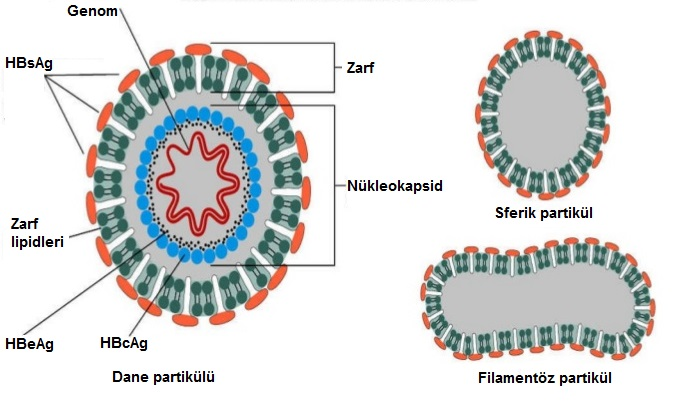
\includegraphics[width=0.6\linewidth]{../Figures/HBVstructure}
\caption[Hepatit B virüsünün yapısı]{Hepatit B virüsünün yapısı \par ({\scriptsize McGraw-Hill Companies Inc'den kaynak alınmıştır})}
\label{fig:HBVstructure}
\end{figure}

\subsection{Hepatit B Virüsü'nün Yapısı, Proteinleri ve Enzimleri}


\textbf{Virion}: DNA genomu, viral kapsid ve bunu saran zarfı içeren 42 mm çaplı enfeksiyoz küresel yapıdır (Dane partikülü).

\textbf{Zarf}: Lipoprotein yapıdadır ve nükleokapsidi çevreler. Membran lipidleri hepatosit membranı kökenlidir. Zarf yüzeyindeki HBsAg ise polipeptid yapıdadır. 

\textbf{Kapsid}: Viral genomu çevreleyen, protein yapılı HBV kapsidi ikozahedral (20 eşkenar üçgen yüz, 12 köşe) simetri göstermektedir. Hepatit B core antijen (HBcAg) ikişer ikişer disülfit bağları ile stabilize olduktan sonra bu birimlerden 180-240 tanesi bir araya gelerek kapsidi oluşturur. 

\textbf{Genom}: Kısmi çift sarmallı sirküler yapıda DNA içerir. Negatif iplikçik tam uzunluktadır, pozitif iplikçik ise kısmi tamamlanmıştır. 

\textbf{HBsAg (Hepatit B surface antijen)}: HBV'nin glikolize zarf proteinidir. Aktif covalently closed circular DNA (cccDNA)'dan ve integre DNA'dan sentezlenir. Büyük (L-HBsAg), orta (M-HBsAg), küçük (S-HBsAg) olmak üzere üç formu vardır (Şekil \ref{fig:hbsag}). S-HBsAg Dane partikülünde en fazla bulunan yüzey proteinidir. Fazla miktarda sentezlenerek hepatositten salınır. 

\begin{figure}[tbph]
\centering
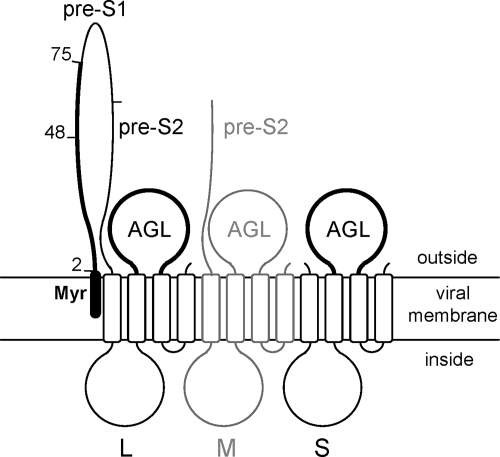
\includegraphics[width=0.45\linewidth]{../Figures/hbsag}
\caption[HBsAg'nin şematik görünümü]{HBsAg'nin şematik görünümü \cite{le2009pre} {\scriptsize \par AGL: Antigenic loop, Myr: Myristic acid}}
\label{fig:hbsag}
\end{figure}

\newpage

\textbf{HBcAg}: Viral DNA'yı çevreleyen kapsidin yapısı oluşturan proteinlerdir. Serumda serbest bulunmaz, hepatosit yüzeyinde eksprese edildiğinden immun yanıt oluşturur. 

\textbf{HBeAg (Hepatit B envelope antijen)}: Replikasyon için gerekli değildir, tam fonksiyonu bilinmemektedir. Hepatositten dışarı salınır. Viral DNA sentezlenmesinde kalıp olarak kullanılan pregenomik RNA (pgRNA)'dan sentezlendiğinde fazla saptanması, fazla miktarda pgRNA sentezlendiğini yani viral replikasyonun ve infektivitenin yüksek olduğunun göstergesidir. 

\textbf{HBV DNA polimeraz enzimi}: DNA polimeraz, revers transkriptaz ve RNase aktivitesi vardır. 

\textbf{HBx}: HBV replikasyonunda rol oynar, HBV'nin onkojenik potansiyaline katkıda bulunduğu bildirilmiştir \cite{liang2009hepatitis}.


\subsection{Hepatit B Virüsü'nün Genomu}

Genom, kısmi çift sarmallı sirküler yapıda ve yaklaşık 3,2 kb uzunluğundadır. Negatif iplikçik tamamlanmıştir, pozitif iplikçik ise değişen uzunluklardadır ve negatif iplikçikten daha kısadır. Negatif ipçiğin 5' ve 3' uçları arasında boşluk vardır ve negatif ipçik pozitif ipçik sayesinde halka şeklinde tutulur. Viral genomun bu yapısı gevşek sirküler DNA (rcDNA) olarak adlandırılır. Olgun virion içinde genom bu formdadır, replikasyon sırasında ise cccDNA; yeni oluşan kapsidlerin içinde ise polimeraz enzimi ile birlikte bulunan pgRNA formu halinde bulunur \cite{enfeksiyonlar3willke}.

HBV DNA üst üste binmiş 4 ORF (opening reading frame) içerir (Şekil \ref{fig:hbvgenom}):

\textbf{S (surface) geni}: Üç farklı zarf glikoproteini kodlar: Pre S1 (L-HBsAg), pre S2 (M-HBsAg) ve S proteini (S-HBsAg-Australia Antijen). 

\textbf{C (core) geni}: HBcAg ve HBeAg'yi kodlar.

\textbf{P (polimeraz) geni}: DNA polimerazı kodlar.

\textbf{X geni}: HBx'i kodlar. 


HBV'nin 10 genotipi (A-J) ve multipl subgenotipleri vardır. Farklı HBV izolatları \%90-\%98 aynı nükleotid sekansına sahiptir \cite{jawetz2013adelberg}. Ülkemizde baskın genotip Akdeniz ülkelerinde olduğu gibi genotip D'dir.

\bigskip

\begin{figure}[tbph]
\centering
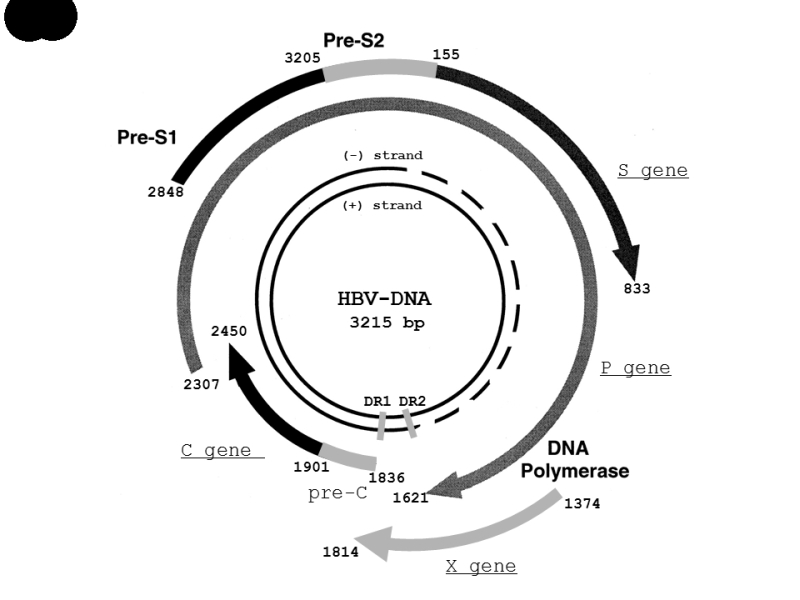
\includegraphics[width=0.7\linewidth]{../Figures/hbvgenom}
\caption[Hepatit B virüsünün genomu]{Hepatit B virüsünün genomu \cite{inoue2016hepatitis}}
\label{fig:hbvgenom}
\end{figure}

\subsection{Hepatit B Virüsü'nün Yaşam Döngüsü ve Hepatotropizm}


HBV'nin girişi; virionun hepatosit yüzeyinde bulunan hepatosit spesifik preS1 reseptörüne ve yüzey heparan sülfat proteoglikanlarına düşük afinite ile geri dönüşümlü olarak bağlanmasıyla başlar (Şekil \ref{fig:hbventry}). Virion; L zarf proteinin pre-S1 domaini ile NTCP (Na taurocholate cotransporting polypeptide)'ye bağlanır ve membran füzyonu ile sitoplazmaya kor partikülleri aktarılır \cite{yan2012sodium, watashi2014ntcp}. Hepatosit içine girişin endositoz ve füzyon ile olduğu öne sürülmüştür \cite{urban2010replication}. Viral DNA sitoplazmadan nükleusa girer ve rcDNA, cccDNA'ya dönüşür. cccDNA, konak polimeraz II'yi kullanarak negatif ipçikten viral transkripsiyonu başlatır. HBV'nin mRNA sentezini yöneten dört promoter bölgesi vardır: PreC/C, PreS1, S ve X promoter'leri (Şekil \ref{fig:hbvgenom}). Oluşan viral mRNA'lar sitoplazmaya gönderilir ve endoplazmik retikuluma bağlı ribozomlarda translasyon gerçekleşir. PreC/C bölgesi viral replikasyonun merkezidir ve pgRNA'yı sentezletir. pgRNA'dan HBcAg, HBeAg, polimeraz protenleri sentezlenir ve aynı zamanda pgRNA viral genom sentezi için kalıptır. Oluşan viral polimeraz pgRNA'nın enkapsidasyon dizisine bağlanarak viral kapsid yapımı başlatılır \cite{jeong2000evidence}. RNA'dan DNA sentezlenmesi anlamına gelen revers transkripsiyon yine polimeraz enzimi ile hücre sitoplazmasında viral kapsid içinde gerçekleşir. Negatif ipçik, sonrasında da pozitif ipçik böylece oluştuktan sonra sentezlenmiş HBsAg ile nükleokapsid birleşir, lipid zar kazanılarak hepatositten enfeksiyoz Dane partikülü olarak salınır ya da yeniden cccDNA oluşumu için nükleusa geri dönüştürülür \cite{yang2014persistence}.

Günde ortalama 10$ ^{11} $ yeni virionun meydana geldiği tahmin edilmektedir. Bu fazla ve hızlı virion üretiminin yanında DNA polimeraz enziminin proof reading fonksiyonunun olmaması replikasyon sırasında çok miktarda hata oluşmasında neden olmaktadır. 

\bigskip

\begin{figure}[tbph]
\centering
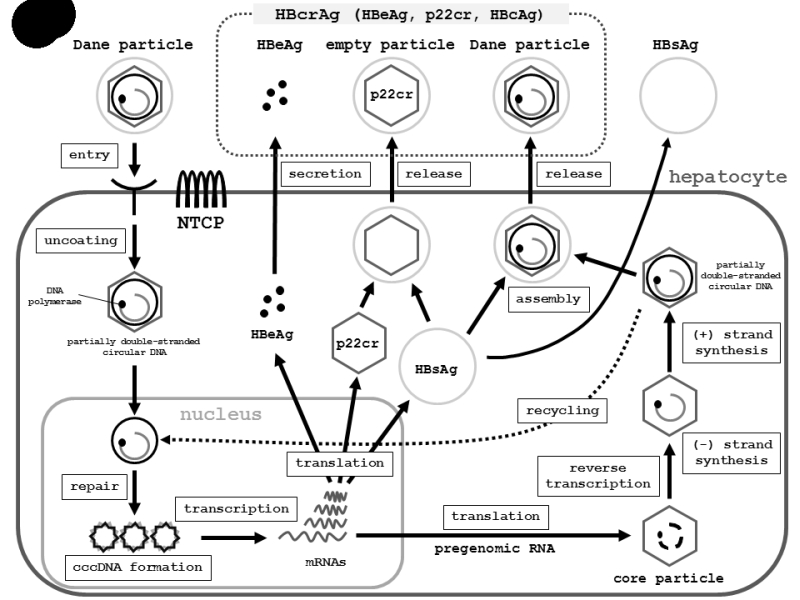
\includegraphics[width=0.9\linewidth]{../Figures/hbventry}
\caption[Hepatit B virüsünün hepatosite girişi, replikasyonu ve salınımı]{Hepatit B virüsünün hepatosite girişi, replikasyonu ve salınımı \cite{inoue2016hepatitis}}
\label{fig:hbventry}
\end{figure}


\subsection{Hepatit B Virüsü'ne Karşı İmmun Yanıt}

HBV’nin primer olarak replike olduğu yer hepatosittir. Direkt olarak sitopatik etkisi yoktur, virüse hücresel ve humoral immun yanıt oluşur. Humoral immun yanıt dolaşan virüs partiküllerini nötralize edip virüsün yayılımını engellemeye çalışırken, sellüler immun yanıt da enfekte hepatositleri öldürür \cite{chisari2010pathogenesis}. HBV, hücre yüzeyi ve endozomda Toll-like reseptörler ile, sitoplazmada da RIG-I (retinoic acid inducible gene I) ve MDA5 (melanoma differentiation gene 5) gibi sensörlerle immun sistem tarafından tanınır ve hepatosit, muhtemelen de diğer hücrelerden IFN salınır, aynı zamanda IFN ile stimule olan genler eksprese edilir \cite{sato2015rna,boeijen2017hepatitis}. Fakat HBV ile indüklenmiş bu IFN yanıtı zayıftır, hatta hayvan çalışmalarında HBV'nin IFN ekspresyonunu indüklemediği gösterilmiştir ve HBV'nin "gizlenen" bir virüs olduğu belirtilmiştir \cite{wieland2005stealth,wieland2004genomic}. Nukleusa cccDNA olarak adapte olmak da bu gizliliğe katkıda bulunur. Hangi patern tanıma reseptörlerinin ya da sinyal yolağının virüsün erken kontrolünde esas rolü oynadığı henüz bilinmemektedir.

Konak immun yanıtında karaciğer sinüzoidlerinde bulunan Kupffer hücreleri ve dendritik hücrelerin naif CD4+ ve CD8+ T hücrelerine antijen sunması da rol oynar ve yanıt aktivasyon ya da tolerans olarak gösterilir. 

Virüsle enfekte hepatositi tanıyan ve lizise uğratan naturel killer hücreler aynı zamanda IFN $ \gamma $ salgılayarak HBV'nin virüse spesifik CD8+ T hücreleri tarafından non sitolitik yolla temizlenmesini düzenler. Ayrıca cccDNA'nın integrasyonun engelleyen antiviral APOBEC ptoteinlerinin yapımı indüklenir.

Virüse spesifik CD4+ ve CD8+ T hücreleri, B hücreleri ve antikorlar HBV kontrolünde vazgeçilmezdir. HBV'ye karşı bu edinilmiş bağışıklık maruziyet sonrası 10 ila 12 haftada gelişir \cite{bertoletti2016adaptive,webster2000incubation}. Bu geç yanıtın virüsün gizli kalma doğasına katkıda bulunduğu düşünülmektedir ama kronikleşmede tek faktör bu değildir, virüsün kendiliğinden kontrol altına alındığı bireylerin çoğunda sonuçta bu gecikmiş yanıt gözlenmektedir.

Virüse spesifik CD4+ T lenfosit hücre yanıtı HBV kor epitoplarını, daha az olarak da yüzey antijeni, polimeraz ve x proteinini hedef alır. Akut, kontrol altına alınmış enfeksiyonlarda kronikleşmiş enfeksiyonlara göre daha hedefe yönelik ve güçlüdür. HBV'ye özgü CD8+ T hücre cevabı virüs temizlenmesinde ve KC hasar patogenezinde temel rolü oynamaktadır. Hepatositler tarafından viral antijenlerin CD8+ lenfositlere sunulmasıyla başlayan sitotoksik T hücre yanıtı enfekte hepatositi apoptoz ile öldürür, aynı zamanda IFN $ \gamma $ sekresyonunu uyarır. Akut hepatitte güçlüdür ve poliklonaldır kronik enfeksiyonda ise zayıftır. Zayıf sitotoksik T hücre yanıtı enfekte hepatositlerin temizlenmesinde yetersiz kalır ama yetersiz persistan hepatosit hasarı devam eder \cite{chisari2010pathogenesis}.


Erken çocuklukta virüse maruziyet ile oluşan kronik enfeksiyon, genellikle yüksek viremiye rağmen karaciğer hasarının bariz olmadığı immuntoleran faz ile karakterizedir. Bu fazda öne sürülen T hücre yanıtının ve/veya işlevinin olmadığıydı. Kronik HBV mekanizması ve immuntolerans sebebi net anlaşılamamakla birlikte sürekli antijen maruziyeti ile CD8+ T hücrelerinin fonksiyonlarının azalması/tükenmesi, inhibitör reseptörlerin ekspresyonu, sitokin proliferasyon kapasitesinin azalması,  viral yük, B ve T lenfosit inaktivasyona yol açan kaçış mutasyonları, viral antijenlerin kazanılmış immun cevabı baskılaması üzerinde durulmaktadır \cite{raziorrouh2010immunoregulatory,schurich2011role,chen2004function,webster2004longitudinal,reignat2002escaping}.



\section{HEPATİT B VİRÜS ENFEKSİYONU}

HBV; enfekte kişiden kan ve vücut sıvıları (semen, tükürük, servikal sekresyonlar, göz yaşı) ile penetran travma ya da mukozal temas ile bulaşabilmektedir. Yüksek prevelanslı bölgelerde HBV’nin enfekte anneden bebeğe perinatal geçişi en sık bulaş yoludur. Düşük prevelanslı bölgelerde ise çocuk doğurma çağındaki kadınlarda HBV enfeksiyon oranının az olmasıyla perinatal bulaş düşüktür ve bu bölgelerde bulaş genellikle adölesan ve yetişkin dönemde seksüel temas, iv ilaç kullanımı, enfekte kan ve kontamine aletlerle olmaktadır. 


HBV infeksiyonunun kliniği ve seyri virüs replikasyonu ve buna karşı immmun sistem yanıtı ile şekillenir. Virüse karşı kuvvetli immun yanıt ile akut-kendini sınırlayıcı hepatit; aşırı ve kontrolsüz yanıt ile fulminan hepatit kliniği oluşabilir. Yetersiz yanıt, tolerans ile virüsün temizlenememesi sonrası HBV kronikleşebilir. Perinatal dönemde HBV’ye karşı immun sistemin tolerans göstermesiyla akut hepatit B tablosundan ziyade kronikleşme görülmektedir böylece siroz ve HCC riski daha fazladır. Adölesan, yetişkin dönemde HBV infeksiyonunda enfeksiyonu akut kendini sınırlayan klinikle ortaya çıkmaktadır ve kronikleşme az; dolayısıyla siroz, HCC riski düşüktür (Şekil \ref{fig:akuthbv}) . 


\begin{figure}[tbph]
\centering
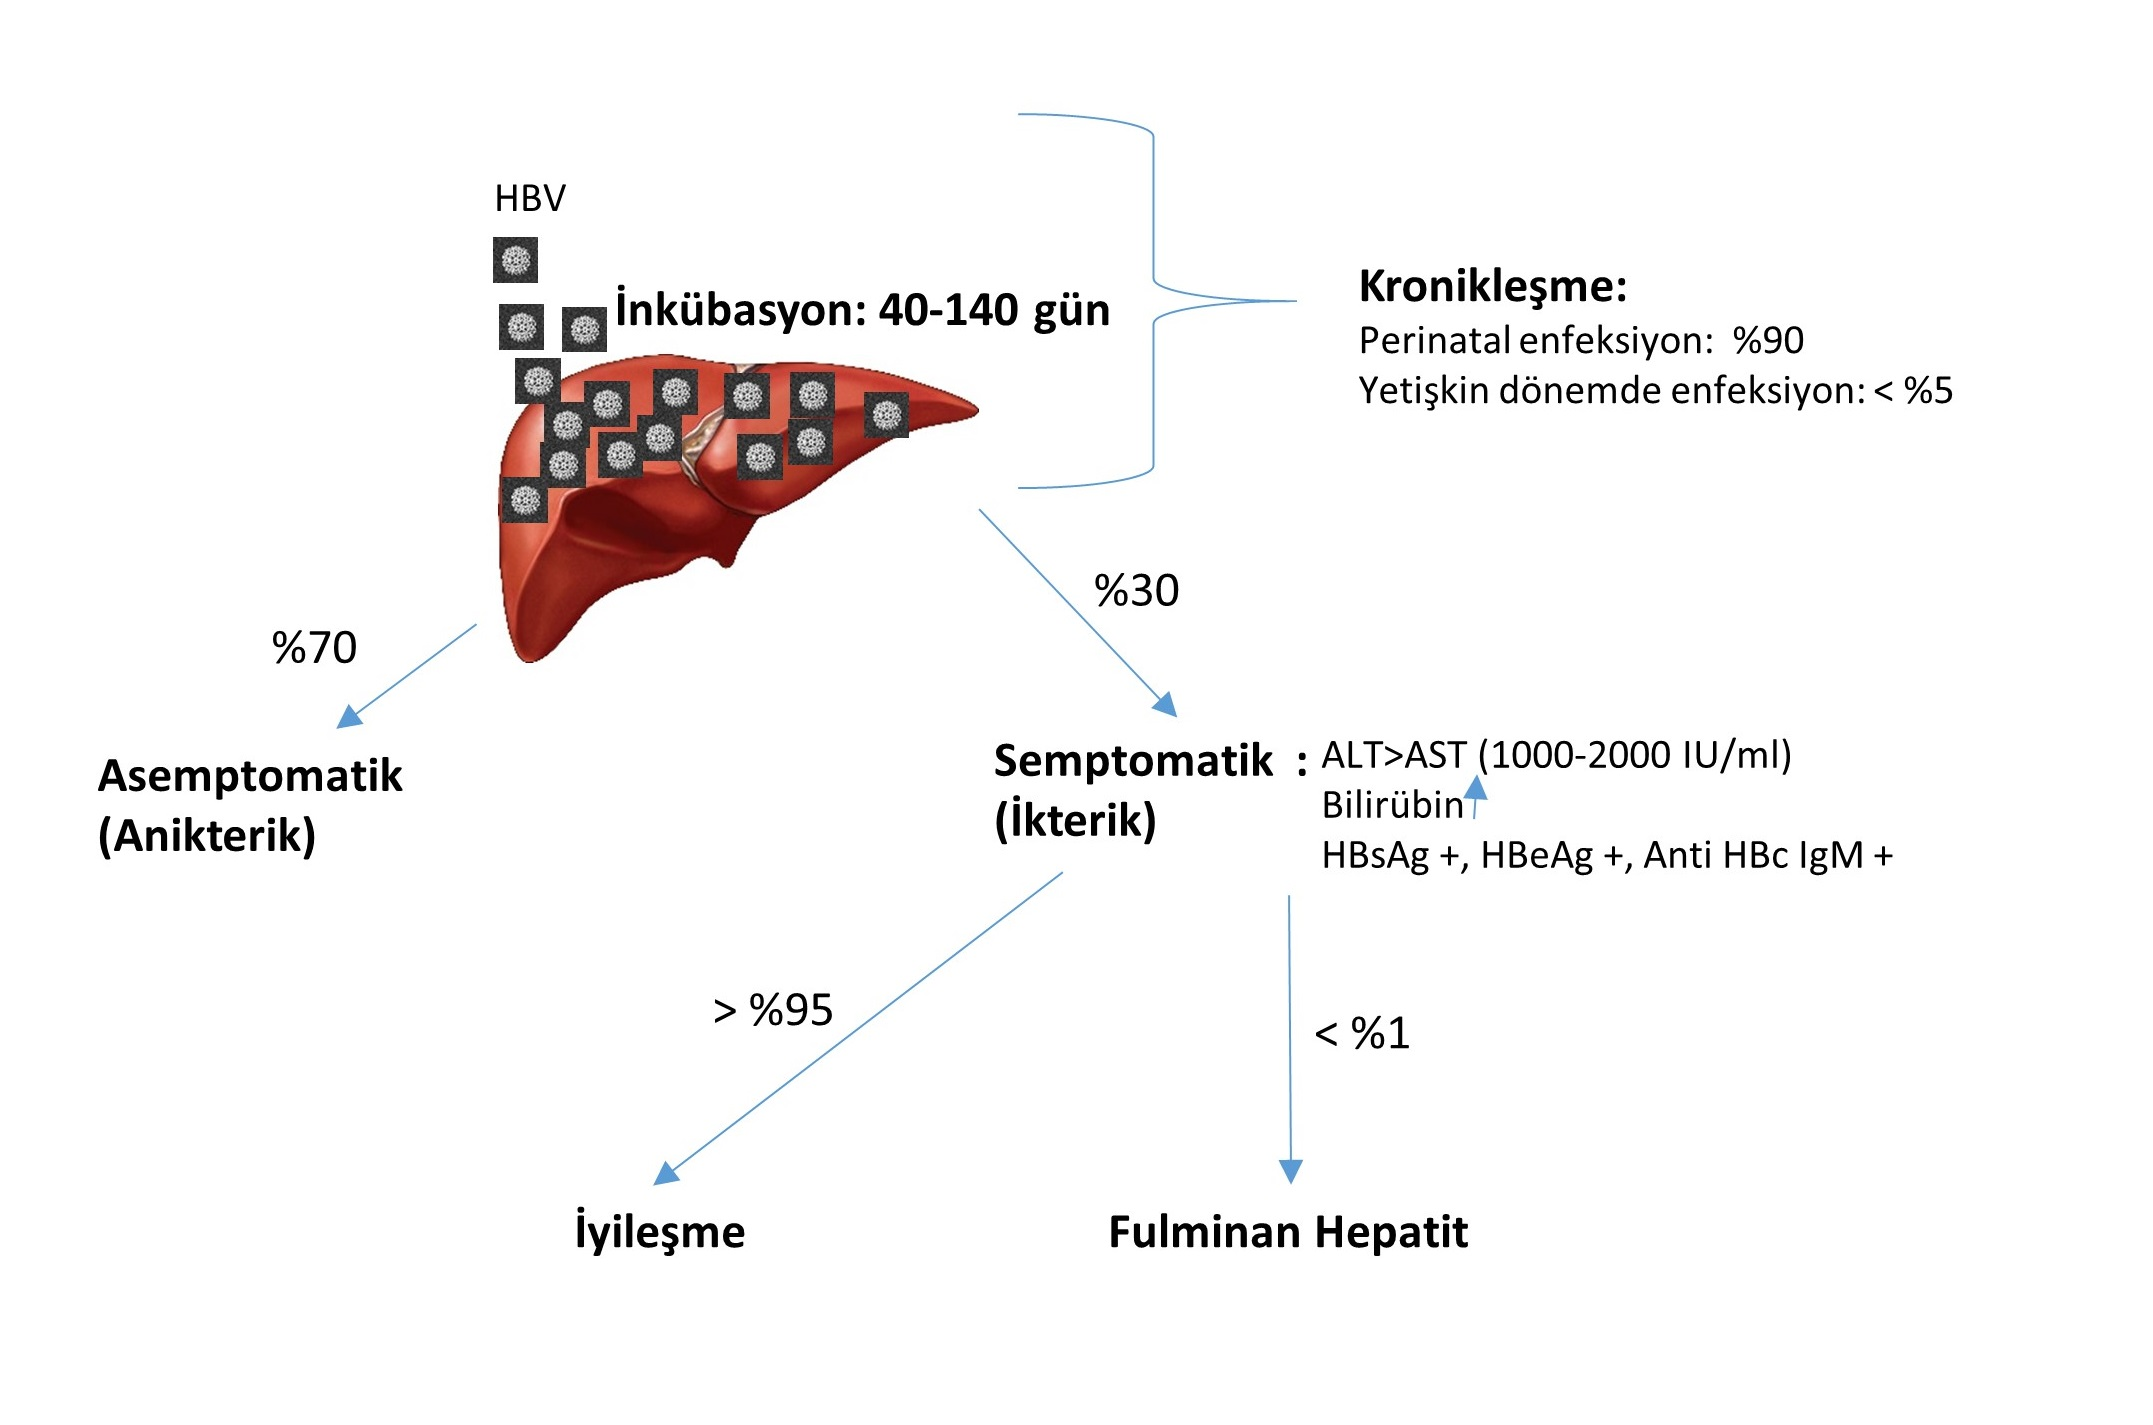
\includegraphics[width=0.8\linewidth]{../Figures/akuthbv}
\caption[Akut HBV enfeksiyonu]{Akut HBV enfeksiyonu \cite{terrault2016aasld}}
\label{fig:akuthbv}
\end{figure}



\subsection{Kronik Hepatit B}

HBsAg'nin 6 ayın üzerinde kanda pozitif saptanmasına kronik hepatit B (KHB) enfeksiyonu tanımlaması yapılmıştır. KHB'nin doğal seyri, HBV replikasyonu ve buna karşı immun yanıtımız çerçevesinde "kronik enfeksiyon" ve "hepatit" kavramları üzerinde yoğunlaşılarak beş faza ayrılmıştır \cite{european2017easl}. Fazların seyri karışıktır, sırayla olmayabilir, bir hastada her faz görülmeyebilir, fazlar arasındaki geçiş süreleri her hastada aynı değildir. Genelde erken yaşlarda enfekte olan kişilerde geçerlidir. 

\textbf{HBeAg pozitif kronik HBV enfeksiyonu (İmmuntoleran Faz):} Esas olarak doğum sırasında ya da erken çocukluk dönemde, nadiren de sonraki yıllarda bulaş ile ortaya çıkmaktadır. Konağın immuntoleransı sebebiyle HBV olabildiğince replike olmakta fakat immun yanıt gelişmediğinden KC'de nekroinflamasyon ve fibrozis oluşmamaktadır. HBeAg pozitif, HBV DNA yüksek, ALT normaldir. KC biyopsisinde inflamasyon/fibroz yoktur ya da minimaldir. Bulaştırıcılık yüksektir. Bu fazın süresi değişkendir, virüsün perinatal kazanımında en uzundur. Yüksek düzeyde HBV DNA integrasyonu olduğundan karsinogenez başlamış olabilir \cite{mason2016hbv}.

\textbf{HBeAg pozitif kronik hepatit B (İmmun Reaktif Faz):} İmmun sistemin reaksiyon göstermeye başlamasıyla hepatosit nekroinflamasyonu başlamıştır. HBeAg pozitiftir, HBV DNA immuntoleran faza göre azalmış olmakla birlikte yüksektir. ALT, immun yanıt ile hepatosit lizisi olduğundan yüksektir. KC'de orta-yüksek nekroinflamatuar aktivite vardır. Fibroza gidiş hızlanmıştır. İmmuntoleran fazdan bu faza geçişin 20'li ya da 30'lu yaşlarda olması beklenmektedir.  Çoğu hasta HBe serokonversiyonu ve HBV DNA baskılanmasıyla HBe negatif kronik HBV enfeksiyonu fazına geçer.

\textbf{HBeAg negatif kronik HBV enfeksiyonu (İnaktif taşıyıcılık):} HBeAg negatif, Anti-HBe pozitif, serum HBV DNA saptanamaz ya da düşük düzeyde, sürekli normal ALT düzeylerinde karaciğer histopatolojisinde hasar yok ya da minimaldir.

\textbf{HBeAg negatif kronik hepatit B: } Anti-HBe oluşmuştur, HBV DNA ve ALT yüksektir. Dalgalı seyir görülebilir, hepatik inflamasyon devam etmektedir. Çoğu vakada kor/prekor mutasyonu sebebiyle HBeAg eksprese edilememektedir.

\textbf{HBsAg negatif faz:} HBsAg negatif, Anti-HBe negatif ya da pozitiftir. ALT genelde normal, HBV DNA saptanamaz düzeydedir. HBsAg seroklirensi sirozdan önce olduysa siroz, HCC riski düşüktür. İmmunsupresyon ile reaktivasyon riski bu hasta grubunda mevcuttur.  


KHB'de antiviral ilaçların kullanım amacı kronik zamanda siroz ve hepatoselüler karsinoma ilerleyişi yavaşlatmak ve bunlara bağlı ölümü engellemektir. Akut hepatit durumunda antiviral tedavinin fulminan hepatite gidişi önleyip önlemediği tartışmalıdır. Şu an elimizdeki antiviral ilaçlar HBV replikasyonunu baskılayabilmektadır; HBV DNA'nın konak genomuna entegre olması, hepatosit nükleusu içindeki cccDNA'nın güncel antiviral ilaçlar ile inhibe edilememesi, HBV'ye karşı immuntolerans (örn. immuntoleran hastalar) gibi sebeplerle eradikasyon ya da kür sağlanamamaktadır  \cite{locarnini2015strategies}.


\subsection{HBeAg Negatif Kronik HBV Enfeksiyonu (İnaktif Taşıyıcılık)}

1987'de Hoofnagle ve arkadaşları HBsAg (+) hastaları kronik hepatit B ve asemptomatik veya sağlıklı taşıyıcı hastalar olarak iki gruba ayırmıştır \cite{hoofnagle1987chronic}. Yapılan çalışmalarda HBsAg (+) bireylerin çoğunda ALT düzeyinin normal olduğu görülmüş, fibrozu saptamak için her hastaya invaziv girişim yapmanın zor, anlamsız olması ve maliyet etkin olmaması HBV DNA için eşik değer arayışlarına yöneltmiştir. 2000'de National Institute of Health tarafından asemptomatik veya sağlıklı taşıyıcılık yerine inaktif HBsAg taşıyıcılığı terminolojisi kullanılmaya başlanmış ve 20000 IU/mL değeri aktif/inaktif hepatit için eşik değeri olarak belirlenmiştir \cite{lok2001management}. Fakat seri HBV DNA ölçümleri ile HBeAg negatif KHB hastalarının yanlış olarak inaktif taşıyıcı olarak değerlendirildiğine dair çalışmalar sonucu eşik değer 2000 IU/mL'ye indirilmiştir \cite{chu2002quantitative,cacciola2005virological}.


Günümüzde, ALT düzeyi normal, HBeAg negatif, Anti-HBe pozitif, HBV DNA saptanamaz ya da düşük seviyede (<2000 IU/ml) olan hastalar ile HBV DNA >2000 IU/mL olup  (genelde 20000 IU/ml'nin altında) ALT düzeyi devamlı normal, karaciğer biyopsisinde minimal nekroinflamatuar aktivite ve düşük fibroz olan hastalar bu fazda olarak değerlendirilir \cite{european2017easl,terrault2016aasld,sarin2016asian}. 


\subsection{HBeAg Negatif Kronik HBV Enfeksiyonunda Komplikasyonlar}

HBeAg negatif kronik HBV enfeksiyonunda antiviral ilaç endikasyonu yoktur. Doğru olarak tanı konduğunda uzun vadede prognoz iyidir, en çok görülecek senaryo yıllar boyu kronik KC hastalığı komplikasyonu olmadan takiptir. Yine de reaktivasyon, siroz ve HCC nadir ama mümkün komplikasyonlardır.    

\textbf{REAKTİVASYON:} Serum HBV DNA'nın yeniden yüksek değerlere ulaşması ve karaciğerdeki nekroinflamatuar aktivitenin artması ile bunun ALT yükselmesi olarak laboratuvara yansımasıdır. HBeAg yeniden pozitifleşebilir. Alevlenmelerle KC'de fibroz düzeyi artabilir. HBV reaktivasyonu kendiliğinden ya da immunsupresif tedavi ile olabilir. HAV, HCV, HDV, HEV ile süperenfeksiyon ve diğer viral hepatit dışı sebepler (ilaç, alkol vb) akılda tutulmalıdır. Kemoterapötik ajanlar (öz. rituksimab ve antrasiklin grubu), kortikosteroidler, metotreksat ve anti-TNF$ \alpha $ kullanımı ile reaktivasyon ve hepatik dekompansasyon riski vardır \cite{yeo2006diagnosis,yeo2008hepatitis,xuan2014hepatitis}. ALT'deki 2 kat artış ile birlikte HBV DNA'nın >20000 IU/ml'nin sonuçlandğı veya saptanabilir HBV DNA düzeyinin reaktivasyon olarak kabul edildiği çeşitli çalışmalarda insidans 0.4 ile 4.7 arasındadır \cite{martinot2002serum,papatheodoridis2008longitudinal,chu2007spontaneous,kumar2009spontaneous,tong2013hepatitis,zacharakis2008role}.


\textbf{FİBROZ/SİROZ:} Yıllarca süren kronik immun yanıt ile hepatosit destruksiyonu ve rejenerasyon siklusları fibroz, siroz ve HCC'ye sebep olur. İnaktif taşıyıcılık tanımında KC'de nekroinflamatuar aktivitenin olmadığı ya da minimal olduğu kabul edilmiştir. Böylelikle bu fazda olduğu kabul edilmiş hastalara KC biyopsisi önerilmez. Fakat yapılan çeşitli çalışmalarda ALT ve DNA düzeyine göre inaktif kabul edilmiş hastaların \%10'unda KC hasarının atlanabileceği görülmüştür \cite{villa2011natural,papatheodoridis2012follow}. Bu hasar doğal klinik seyirdeki HBeAg (+) KHB fazında oluşmuş olabilir. 


\textbf{HEPATOSELÜLER KARSİNOM:} HCC tüm dünyada en sık görülen kanserlerde altıncı sırada olup kanser ile ilişkili mortalitenin üçüncü sebebidir. Etyoloji coğrafi farklılık göstermektedir. Uzakdoğu ve sahra altı Afrika'da daha erken yaşta gelişir ve genetik faktörler, HBV ve ek karsinogenler ile ilişkilidir, batıda ise genellikle geç yaşlarda ve siroz zemininde gelişir. Doubling time 4-6 aydır.   Taraması biyokimyasal ve radyolojik tetkiklerle yapılmaktadır, tanısı ise MR'daki tipik görüntü paterniyle ve/veya biyopsi ile konur. Biyokimyasal testlerden genelde AFP çalışılmıştır. Dünyadaki HCC vakalarının \%50-55'i, endemik bölgelerdeki HCC vakaların ise \%70-80'i HBV'ye atfolunur. Siroz, HCC için öncü kliniktir fakat KHB hastalarının yılda yaklaşık \%0.1'inde siroz olmadan da HCC gelişebilir \cite{fattovich2008natural,chayanupatkul2017hepatocellular}. HCC oluşumunda çok sayıda HBV'ye ve hastaya bağlı faktör rol oynar. Konak genomuna entegre olmuş HBV DNA ve mikrodelesyonlar hücresel bölünme kontrol mekanizmalarını bozarak onkogen etkisi gösterebilir \cite{matsubara1990integration}. Buna ek olarak bazı HBV proteinleri direkt olarak HCC gelişiminde rol oynayabilir. HHBx'in çeşitli transkripsiyon faktörleri, tümor supresyon genleri ve DNA tamirinde rol alan proteinlerle  etkileşimde bulunduğu gösterilmiştir \cite{chisari2010pathogenesis,kremsdorf2006hepatitis}.

İnaktif taşıyıcılarda HBV DNA saptanamaz düzeyde olsa bile, HBV ile enfekte olmayan populasyona göre HCC riski daha fazladır \cite{chen2010carriers}. İleri yaş, ailede HCC öyküsü, siroz varlığı, alkol kullanımı, HBV DNA yüksekliği, ALT yüksekliği, HBe serokonversiyon süresinin uzaması HCC gelişimi için risk faktörleridir. HBsAg serokonversiyonu sonrası da HCC riski devam etmektedir bu sebeple özellikle serokonversiyon gelişmiş 50 yaş üstü erkek hastalarda HCC taramasının devam etmesi önerilmektedir \cite{yip2017impact}. Diğer HCC taramasının önerildiği KHB taşıyıcı hasta grupları sirotik hastalar, 50 yaş üstü Asya kökenli kadınlar, 40 yaş üstü Asya kökenli erkekler, ailede HCC öyküsü olanlar, Afrikalı-Kuzey Amerikalı siyahiler ve sirozlulardır \cite{bruix2011management}. HCC oranlarının yüksek belirtildiği yayınlar genelde Asya kaynaklıdır (Öz. Tayvan). Bunun nedeni perinatal dönemde kazanılmış HBV, genetik faktörler ve ek karsinojenler olabilir. Düşük düzey DNA ve normal ALT ile uzun süre takip edilen taşıyıcıları içeren Avrupa kaynaklı yayınlarda bu oran daha düşüktür. 

Özellikle riskli gruptaki hastalarda görüntüleme yöntemleri ile tanıda geç kalmamak adına HCC taraması devam etmelidir. Semptomlar çıktığından sonra saptanmış HCC'de 5 yıllık prognoz kötüdür.




\textbf{HBsAg SEROKLİRENSİ:} KHB'de immun kontrolün sağlandığının en iyi serolojik göstergesidir. HBsAg seroklirensi ve Anti-HBs serokonversiyonu genellikle birkaç yıl saptanamaz düzeyde seyreden HBV DNA ölçümlerinden sonra yılda \%1-\%3 hastada görülmektedir \cite{martinot2002serum}.  Seroklirens genç yaşta, fibroz gelişmeden oluştuğunda prognoz mükemmeldir ancak seroklirens esnasında sirozlu hastada klinik kötüye gidiş, dekompansasyon, HCC ve bunlara bağlı ölüm üzerinde etkisi yoktur.   

Tablo \ref{tablo:lit}'de literatürde inaktif taşıcılarda doğal seyir ile ilgili yaplmış çalşmalar gösterilmiştir


%\begin{\begin{landscape}
\begin{sidewaystable}
\begin{minipage}[c]{\textwidth}
\renewcommand{\arraystretch}{1.3} %SATIR ARALI^GI BEL'IRLEMEK 'IÇ'IN SAYIYI DE^G'I¸ST'IR'IN
\centering
\begin{threeparttable}
\caption[HBeAg negatif kronik HBV enfeksiyonunda doğal seyir ile ilgili literatüler]{HBeAg negatif kronik HBV enfeksiyonunda doğal seyir ile ilgili literatürler} \label{tablo:lit} %Tablo ba¸slı^gı ve referans etiketi
%---------------------------------------
{\scriptsize \begin{tabular}{llllL{1cm}L{1.4cm}L{1.4cm}llL{1cm}L{1.7cm}L{1.7cm}}
\toprule\toprule
                         & \textbf{ÜLKE} & \textbf{DİZAYN} & \textbf{N} & \textbf{İZLEM (YIL)} & \textbf{REAKT. N (\%)} & \textbf{REAKT. İNS} & \textbf{S N (\%)} & \textbf{HCC N (\%)} & \textbf{HCC İNS.} & \textbf{HBsAg KLR N (\%)} & \textbf{HBsAg KLR İNS. 100 kişi-yıl} \\
\midrule
Martinot-Peignoux (2002) \cite{martinot2002serum} \tnote{1,  } \:\tnote{a} & Fransa        & Prospektif      & 38         & 3.2                & 1 (1)                  & 0.8                      & 0                & 0                  &                        &                           &                              \\
Martinot-Peignoux (2013) \cite{martinot2013prediction} \tnote{1} \:\tnote{a} & Fransa        & Prospektif      & 54         & 10                 & 0 (0)                  &                          &                  &                    &                        & 8 (15)                    & 1.5           \\
Chen (2010) \cite{chen2010carriers} \tnote{1}            & Tayvan        & Prospektif      & 1932       & 13.1               &                        &                          &                  & 16 (0.82)          & 0.06                   &                           &                              \\
Habersetzer (2015) \cite{habersetzer2015loss}  \tnote{1}    & Fransa        & Prospektif      & 109        & 6                  &                        &                          &                  &                    &                        & 11 (3.5)                  & 2.3         \\
Magalhães (2015) \cite{magalhaes2015hepatitis} \tnote{1} \:\tnote{h}       & Portekiz      & Retrospektif    & 100        & 4.6                & 10 (10)                &                          & 0                & 0                  &                        & 4 (4)                     &                              \\
Tong ve Trieu (2013) \cite{tong2013hepatitis} \tnote{1} \:\tnote{f}    & USA           & Prospektif      & 146        & 8                  & 1 (0.7)                &                          & 0                & 2 (1.3)            & 0.17                   & 13 (9)                    & 1.1            \\
Papatheodoridis (2008) \cite{papatheodoridis2008longitudinal} \tnote{2} \:\tnote{e}   & Yunanistan    & Prospektif      & 85         & 3                  & 12 (14)                & 4.7                      &                  &                    &                        &                           &                              \\
Oliveri (2017)  \cite{oliveri2017long}   \tnote{2} \:\tnote{g}      & İtalya        & Prospektif      & 133        & 4.7                & 1 (0.75)               &                          & 0                & 0                  &                        & 21 (15.7)                 &                              \\
Gigi (2007) \cite{gigi2007long}    \tnote{2} \:\tnote{d}          & Yunanistan    & Retrospektif    & 307        & 7.4                & 73 (23.8)              &                          & 1                & 0                  &                        & 24 (7.8)                  &                              \\
Zacharakis (2008) \cite{zacharakis2008role} \tnote{3} \:\tnote{c}      & Yunanistan    & Prospektif      & 195        & 5.3                & 4 (2.1)                & 0.4                      & 0                & 0                  &                        & 16 (8.2)                  &                              \\
Chu ve Liaw (2007) \cite{chu2007spontaneous}  \tnote{3} \:\tnote{b}     & Tayvan        & Prospektif      & 1241       & 12.3               & 211 (17)               & 1.4                      & 40 (3.2)         & 4 (0.32)         &                        &                           &                              \\
Chu ve Liaw (2007) \cite{chu2007hbsag}  \tnote{3} \:\tnote{b}     & Tayvan        & Prospektif      & 1965       & 10.8               & 314 (15.9)             & 1.55                     &                  &                    &                        & 245 (12)                  & 1.2           \\
Kumar (2009)  \cite{kumar2009spontaneous}   \tnote{3} \:\tnote{a}        & Hindistan     & Prospektif      & 217        & 6.3                & 43 (19.8)              & 3.1                      &                  &                    &                        &                           &                              \\
Hsu (2002)  \cite{hsu2002long}   \tnote{3}          & Tayvan        & Prospektif      & 189        & 8.2                &                        &                          & 1 (0.5)        & 3 (1.6)            &                        & 9 (4.8)                   &                              \\
Taida (2016)  \cite{taida2017prognosis}   \tnote{4}        & Japonya       & Prospektif      & 388        & 2.8                &                        &                          & 0                & 0                  &                        &                           &     \\
\bottomrule                        
\end{tabular}}
%------------------------------------------
\footnotesize
\begin{tablenotes}
\item \textbf{REAKT.}: Reaktivasyon; \textbf{İNS.}: İnsidans; \textbf{S}: Siroz; \textbf{KLR.}: Klirens \par
\textbf{İnaktif Taşıyıcılık Kriteri:} \par
\item [1] HBeAg (-), Anti-HBe (+); ALT N, HBV DNA<2000 IU/ml \par
\item [2] HBeAg (-), Anti-HBe (+), ALT: N, HBV DNA<20000 IU/ml \par
\item [3] HBeAg (-), Anti-HBe (+), ALT:N \par
\item [4] HBeAg (-), Anti-HBe (+), ALT<31 U/L; HBV DNA<4 log kopya/ml \par
\textbf{Reaktivasyon Kriteri:} \par
\item[a] ALT$ \geq $ 2ULN ve/veya HBV DNA>20000 IU/ml \par
\item[b] ALT$ \geq $ 2ULN ve HBV DNA'nın saptanabilir düzeyde olması \par
\item [c] ALT yüksek ve HBV DNA >2000 IU/ml \par
\item [d] ALT yüksek ve HBV DNA >20000 IU/ml \par
\item [e] ALT artışı, saptanabilir HBV DNA ve KHB ile uyumlu histopatoloji \par
\item [f] ALT > 80 U/L ve HBV DNA   $ \geq $ 1000000 kopya/mL \par
\item [g] ALT N ya da yüksek ve HBV DNA >20.000 IU/ml \par
\item [h] Belirtilmemiş


%\item [$\S$] third note ;
%\item [**] the first note;
\end{tablenotes}
\end{threeparttable}
\end{minipage}
\end{sidewaystable}
%\end{landscape}}


\newpage

\subsection{HBeAg Negatif Kronik HBV Enfeksiyonu'nun Takibi}

İlk defa başvurmuş HBsAg pozitif bir hastadan ayrıntılı anamnez alınmalıdır. Bulaş yolu açısından annede ve diğer birinci derece akrabalarda HBsAg pozitifliğinin bilinip bilinmediği, riskli cinsel temas, diyaliz öyküsü, kan ve kan ürünleri nakli, ameliyat öyküsü, diş tedavisi, iv ilaç kullanımı sorgulanmalıdır. Komorbiditeler (obezite, diyabet, metabolik sendrom) değerlendirilmeli, kronik KC hastalığı açısından fizik muayenesi (ödem, ikter, batın kollateralleri, asit muayenesi vb) yapılmalıdır. HBV replikasyonu ve kronik KC hastalığı varlığı açısından hemogram, ALT, AST, ALP, GGT, total ve direkt bilirübin, albumin, protrombin zamanı, HBeAg, Anti-HBe, HBV DNA testleri ile koinfeksiyonlar için Anti-HCV, Anti-HDV, Anti-HIV; hepatit A virüsüne bağışıklığı belirlemek için de Anti-HAV IgG bakılmalıdır. Anti-HAV IgG negatif olanlar aşılanmalıdır. Birinci derece akrabalar ve partnerler de HBV için taranmalı, bağışıklıkları yoksa aşılanmalıdır. 


HBV DNA <2000 IU/ml, HBeAg negatif, ALT düzeyi normal olan bir hastada tek ölçüm ile inaktif taşıyıcılık tanısı konulmamalıdır. HBeAg negatif KHB'de HBV DNA ve ALT dalgalı seyredebileceğinden hastalar ilk yıl içerisinde üç ayda bir ALT ve periyodik olarak HBV DNA düzeyi takip edilmesi önerilmektedir \cite{european2017easl}. İnaktif taşıyıcılık ile HBeAg negatif KHB'nin ayrımı, iki kliniğin seyrindeki farklılık sebebiyle önemlidir. İnaktif taşıyıcılıkta prognoz iyidir, komplikasyonlara ilerleyiş riski düşüktür, HBeAg negatif KHB'de ise bu risk daha yüksektir. 


İlk bir yıllık takipte ALT düzeyi normal seyrediyorsa kontrol periyodu 6 aya çekilebilir. Yapılan çalışmalarda ilk ALT düzeyi normal olan hastaların ilk bir sene içinde yüksek bir ALT düzeyine sahip olma ihtimalinin \%15-20 olduğu görülmüş ve bu riskin 3 senelik takip sonrasında azaldığı gözlenmişir bu yüzden ilk 1-3 yılda yakın gözlem önemlidir \cite{papatheodoridis2012follow,papatheodoridis2008longitudinal}. 


Rehber önerilerine baktığımızda EASL 2017, HBV DNA < 2000 IU/ml olan hastalarda ALT'nin 6-12 ayda bir bakılmasını ve 2-3 yılda bir de KC fibroz durumunun değerlendirmesini; HBV DNA $ \geq $ 2000 IU/ml olan hastalardaysa en az 3 ayda bir ALT ve HBV DNA bakılmasını, her yıl da non invaziv bir test ile KC fibroz değerlendirmesinin yapılmasını önermektedir \cite{european2017easl}.

APASL 2015, HBV DNA < 2000 IU/ml olan hastalarda 3-6 ayda bir ALT ve AFP, 6-12 ayda bir de HBV ve KC USG takibini önermektedir. HBV $ \geq $ 2000 IU/mi ise de 3 ayda bir  HBV DNA ve ALT ile takip önermektedir \cite{sarin2016asian}. 

VHSD 2017 ise, inaktif taşıyıcıların 6-12 ayda bir HBV DNA, AFP ve KC USG ile takip edilmesini önermektedir \cite{vhsd2017}.  

Uzman görüşlerinde HBV DNA > 2000 IU/ml olan hastalara KC biyopsisi yapılabileceği belirtilmektedir. Çeşitli yayınlarda ALT düzeyi normal HBV DNA 2000-20000 IU/ml olan hastaların çok azında belirgin KC hasarı saptanmıştır. Bu hasta grubunda ALT ilk bir yıl 3 ayda bir, sonrasında 6 ayda bir HBV DNA ile değerlendirilmeli ve fibroz da non invaziv olarak senede bir kere üç sene boyunca takip edilmelidir. Üç sene sonrasında tedavi düşünülmüyorsa hayat boyunca diğer hastalar gibi takibe devam edilmelidir \cite{papatheodoridis2012follow}. Eğer ALT yükselir ve HBV DNA $ \geq $ 20000 olursa özellikle 35 yaş üstü ve ailesinde siroz/HCC öyküsü olan hastalarda karaciğerin invaziv ya da noninvaziv değerlendirmesi uygun olacaktır. 

\subsubsection{AFP, Görüntüleme Yöntemleri ve KC biyopsisi}

AFP, yolk kesesi ve fetal KC'den salgılanan bir plazma proteinidir. 8-12 yaştan itibaren yetişkindeki değerine düşer. Aynı endoderm kökenli organların tümörlerinde (HCC, mide kanseri, pankreas kanseri, intrahepatik kolanijokarsinomlar) serum AFP değerleri yükselebildiği gibi; tütün, alkol kullanımı, gebelik, kolon kanseri metastazları, testisin nonseminom germ hücreli tümörlerinde de yükselebilir. Karaciğerde kitle ve AFP yüksekliği direkt olarak HCC varlığını göstermez. HCC taramasında AFP'nin sensitivitesi ve spesifitesi yetersizdir \cite{bruix2011management}.


USG; kolay ulaşılabilirlik, radyasyon içermemesi ve düşük maliyetli olması gibi avantajlarla kronik KC hastalığı ve HCC taramasında kullanılır. Karaciğerin parenkim değerlendirmesi subjektiftir ve siroz tanısında duyarlılığu düşüktür. Birden fazla görüntüleme bulgusunun bir arada olması (parenkim ekosu yaygın kaba, karaciğer yüzeyinin nodüler görüntüsü, asit varlığı) daha kuvvetli olarak siroz düşündürür. HCC tanısında USG'un, BT ve MR'a göre duyarlılığı daha düşüktür ve rejeneratif nodüller, displastik nodüller ile küçük HCC odağı ayırt edilemeyebilir \cite{arif2014mri}.

USG'da 1 cm'den büyük nödül saptandığında 4 fazlı (erken arteryal, arteryal, venöz ve geç fazları içeren) dinamik BT ya da MR çekilmelidir. 1 cm'den küçük nodüllerde 3 ay sonra kontrol USG önerilmektedir, lezyonda büyüme yoksa USG takibi 3-6 ayda bir devam etmeli, boyut büyüdüyse 4 fazlı dinamik BT ya da MR çekilmelidir. HCC portal dolaşımdan kanlanmadığından arteryal hipervaskülarite ve venöz geç fazda kontrast kaybı (washout) görüntüsü HCC tanısı koydurur (Şekil \ref{fig:hcc}).  Bu tipik görüntü yoksa başka bir kontrastlı dinamik görüntüleme (BT ya da MR) çekilmelidir. Yine emin olunamıyorsa biyopsi yapılmalıdır \cite{bruix2011management}. 

\bigskip

\begin{figure}[tbph]
\centering
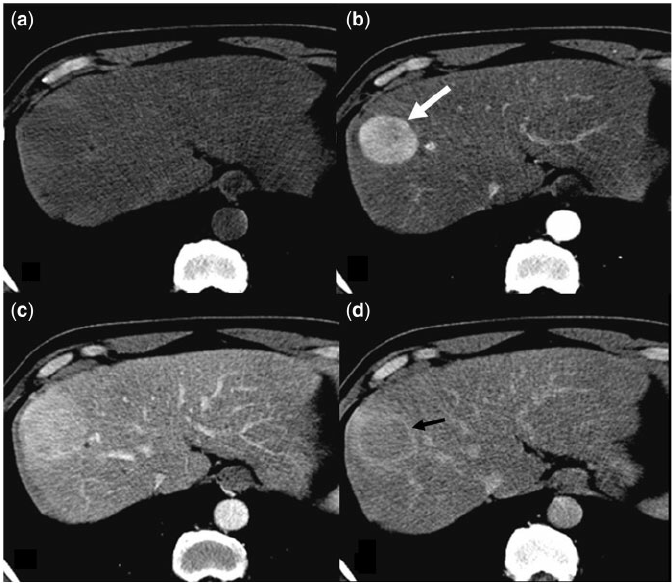
\includegraphics[width=0.7\linewidth]{../Figures/hcc}
\caption[Hepatoselüler karsinoma MR görüntüsü (washout patern)]{KHB'li bir hastada HCC'nin MR görüntüsü (washout patern) \cite{hennedige2012imaging} \par \textbf{(a)} Erken Faz-kontrast tutulumu yok \textbf{(b)} Arteriyel Faz, \textbf{(c)} Portal venöz faz, \par \textbf{(d)} Geç faz. İnce psödokapsül geç fazda görülmekte}
\label{fig:hcc}
\end{figure}


Kontrastlı dinamik MR ile anlatıldığı gibi biyopsi ihtiyacı olmadan tipik görüntü ile HCC tanısı konabilmektedir. >2 cm tümörlerde sensitivite artmaktedır. KC'in en fazla saptanan lezyonu hemanjiom ile ayrımın yapılmasında en iyi görüntüleme yöntemidir. 

Biyopsi KHB'de tanıdan ziyade KC hasarının belirlenmesi ile evrelendirmede ve olası diğer hastalıkların ekartasyonunda kullanılır. Antiviral ilaçlara yanıt ve hastalığın ilerleyişi de kontrol biyopsiler ile değerlendirilebilir. KC biyopsisi, KC'in yaklaşık 1/50.000'ini gösterir. KC'de fibroz heterojenite gösterdiğinden KC dokusunun gerçek durumu atlanabilir, aynı zamanda patologlar arasında değerlendirme farklılığı da bulunabilir. Biyopsi sonrası komplikasyonların yarısından fazlası ilk 2 saatte, neredeyse tamamı ilk 24 saat içinde olmaktadır. Bunlar sıklıkla ağrı, kanama, vazovagal refleks veya kanama ile açıklanabilecek hipotansiyon, yanlış anatomik bölgeye girilmesi sebebiyle oluşabilecek pnömotoraks, hemotoraks, safra kesesi perforasyonu, hemobili, pnömoperitoneumdur. Nondiagnostik biyopsi de bir diğer sorundur. Alınan parça en az 11 portal alan içermelidir bu da 16 gauge iğne kullanılarak alınmış en az 2 cm uzunluğundaki biyopsi materyali ile mümkün olur \cite{standish2006appraisal}. 

Biyopside patoloji tarafından KC'de nekroinflamasyon (Grade - Derecelendirme - Histolojik Aktivite İndeksi) ve fibroz (Stage - Evreleme) skoru verilir (Tablo \ref{tablo:ishakhai}), (Tablo \ref{tablo:ishakfib}). Bu skor ile takip ve tedavi yaklaşımı belirlenir. Histolojik aktivite indeksi KC'deki inflamasyon ve hepatoselüler hasarın göstergesi olup bu hasarın fibroza ilerleyebileceğini düşündürür. Evre ise fibrozun varlığını ve yaygınlığını gösterir \cite{guido2011chronic}.  

\bigskip

\begin{figure}[tbph]
\centering
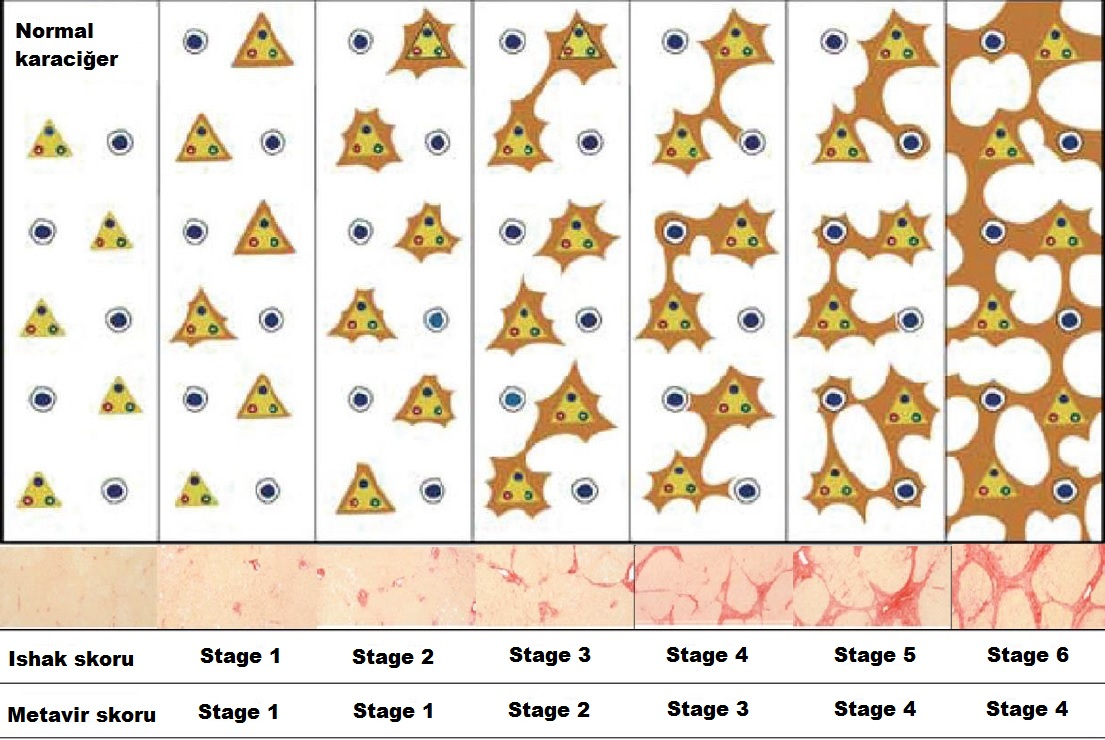
\includegraphics[width=0.9\linewidth]{../Figures/pato}
\caption[Ishak ve Metovir fibroz evrelemesi]{Ishak ve Metovir Fibroz Evrelemesi \cite{guido2011chronic,standish2006appraisal}}
\label{fig:pato}
\end{figure}






%\begin{\begin{landscape}
\begin{minipage}[c]{\textwidth}
\renewcommand{\arraystretch}{1.1} %SATIR ARALI^GI BEL'IRLEMEK 'IÇ'IN SAYIYI DE^G'I¸ST'IR'IN
\centering
\begin{threeparttable}
\caption[ISHAK skorlama sistemine göre modifiye
histolojik aktivite indeksi derecelendirmesi]{ISHAK skorlama sistemine göre modifiye
histolojik aktivite indeksi derecelendirmesi} \label{tablo:ishakhai} %Tablo ba¸slı^gı ve referans etiketi
%---------------------------------------
{\scriptsize \begin{tabular}{ll}
\toprule\toprule
\textbf{A. Periportal veya periseptal interface hepatiti (*piecemeal*)}              &   \\
\midrule
Yok                                                                                  & 0 \\
Hafif (fokal, birkaç portal alanda)                                                  & 1 \\
Hafif/Orta ( fokal, portal alanların çoğunda)                                        & 2 \\
Orta (trakt ya da septaların \%50’den azında, çevresinde devamlılık gösteren)        & 3 \\
Şiddetli (trakt ya da septaların \%50’den fazlasında, çevresindedevamlılık gösteren) & 4 \\
\midrule
\textbf{B. Konfluent nekroz}                                                         &   \\
\midrule
Yok                                                                                  & 0 \\
Fokal konfluent nekroz                                                               & 1 \\
Zon 3 nekroz (bazı alanlarda)                                                        & 2 \\
Zon 3 nekroz (çoğu alanda)                                                           & 3 \\
Zon 3 nekroz + seyrek portal-santral (P-C) köprüleşme                                & 4 \\
Zon 3 nekroz + çok sayıda portal-santral (P-C) köprüleşme                            & 5 \\
Panasiner veya mültiasiner nekroz                                                    & 6 \\
\midrule
\textbf{C. Fokal (*spotty*) litik nekroz, apoptozis fokal inflamasyon}               &   \\
\midrule
Yok                                                                                  & 0 \\
1 veya daha az odak (x 100’lik her büyütmede)                                        & 1 \\
2-4 odak (x 100’lük her büyütmede)                                                   & 2 \\
5-10 odak (x100’lük her büyütmede)                                                   & 3 \\
10’dan fazla odak (x100’lük her büyütmede)                                           & 4 \\
\midrule
\textbf{D. Portal inflamasyon}                                                       &   \\
\midrule
Yok                                                                                  & 0 \\
Hafif (bazı veya tüm portal alanlarda)                                               & 1 \\
Orta (bazı veya tüm portal alanlarda)                                                & 2 \\
Orta/Belirgin (tüm portal alanlarda)                                                 & 3 \\
Belirgin (tüm portal alanlarda)                                                      & 4 \\
\bottomrule
\end{tabular}}
%------------------------------------------
\begin{tablenotes}
%\footnotesize
%\item [*] Bazı hastalarda 2000-20000 IU/ml aralığında olup, ALT normal, KC hasarı yok/minimaldir.
%\item [**] Dalgalı seyir
%\item [$\dag$] second note ; %tabloya "\tnote{*}" ekleyin
%\item [$\ddag$] third note ;
%\item [$\S$] third note ;
%\item [**] the first note;
\end{tablenotes}
\end{threeparttable}
\end{minipage}
%\end{landscape}}



\bigskip

%\begin{\begin{landscape}
\begin{minipage}[c]{\textwidth}
\renewcommand{\arraystretch}{1.1} %SATIR ARALI^GI BEL'IRLEMEK 'IÇ'IN SAYIYI DE^G'I¸ST'IR'IN
\centering
\begin{threeparttable}
\caption[ISHAK skorlama sistemine göre fibrozis evrelemesi]{ISHAK skorlama sistemine göre fibrozis evrelemesi} \label{tablo:ishakfib} %Tablo ba¸slı^gı ve referans etiketi
%---------------------------------------
{\scriptsize \begin{tabular}{ll}
\toprule\toprule
\textbf{}                                                                                                        & \textbf{Skor} \\
\midrule
Fibrozis yok                                                                                                     & 0             \\
Birkaç portal alanda fibröz genişleme ve +/- kısa fibröz septa                                                   & 1             \\
Portal alanların çoğunda fibröz genişleme ve +/- kısa fibröz septa                                               & 2             \\
Portal alanların çoğunda fibröz ve seyrek portal –portal (P-P) köprüleşme                                        & 3             \\
Portal alanlarda fibröz genişleme ve belirgin köprüleşme{[}Portal-portal (P-P) yanı sıra portal-santral (P-C){]} & 4             \\
Belirgin köprüleşme (P-P ve/veya P-C) ile seyrek nodül (inkomplet siroz)                                         & 5             \\
Siroz (olası veya kesin)                                                                                         & 6      \\
\bottomrule    
\end{tabular}}
%------------------------------------------
\begin{tablenotes}
%\footnotesize
%\item [*] Bazı hastalarda 2000-20000 IU/ml aralığında olup, ALT normal, KC hasarı yok/minimaldir.
%\item [**] Dalgalı seyir
%\item [$\dag$] second note ; %tabloya "\tnote{*}" ekleyin
%\item [$\ddag$] third note ;
%\item [$\S$] third note ;
%\item [**] the first note;
\end{tablenotes}
\end{threeparttable}
\end{minipage}
%\end{landscape}}
     

Yukarıda belirtilen dezavantajlar sebebiyle biyopsiye olan ihtiyacı azaltmak ve biyopsinin kontrendike olduğu hastalarda KC fibrozu değerlendirmesinde ultrasonografik ileri görüntüleme yöntemleri ön plana çıkmaktadır. Bunlar transient elastografi, akustik radyasyon kuvveti impulsu görüntülenmesi (ARFI), shear dalgası elastografisi (SWE)'dir. Temel prensip dokunun sertliğini tespit etmektir.

Transient elastografide KC'e düşük frekanslı ve amplitüdlü titreşimler gönderilir. Eğer KC dokusunun esnekliği azalmış, sertliği artmışsa dalganın yayılım hızı artar ve bu hız probdaki dedektör ile saptanıp kilopaskal (kPA) cinsinden ifade edilerek fibroz miktarı belirlenir. 1.5-2.5 ile 75 kPA aralığında sonuç bildirilerek F0'dan F4'e kadar fibroz rapor edilir. Kolay uygulanabilir olması, biyopsi ile karşılaştırıldığında yaklaşık 100 kat daha fazla karaciğer parankimini taraması, komplikasyonsuz olması ve uygulayan kişiler arasında farklılığın az olması yöntemin avantajlarını oluştururken, orta derece fibrozisi ayırt etmede sensitivite ve spesifitesinin tam bilinmemesi, asitli hastalarda ve obez hastalarda ölçüm kalitesini bozulması dezavantajlarını oluşturmaktadır. Gebelerde ve implantı olan hastalarda kullanılması önerilmez \cite{alahdab17transient}.


\subsubsection{Sağlıkta Uygulama Tebliği'ne göre KHB tedavisi}
Takip ve yapılan tetkikler sonrasında KHB tedavisi düşünülürse güncel SGK Sağlıkta Uygulama Tebliği şu şekildedir:

\begin{itemize}
\item İlk tedaviye başlamak için; HBV DNA seviyesi 10.000 kopya/ml (2.000 IU/ml) veya üzerinde olan erişkin hastalara, bu durumun belirtildiği rapor ve eki tetkik sonuçlarına (HBV DNA sonucu ve karaciğer biyopsi raporu) göre karaciğer biyopsisinde Histolojik Aktivite İndeksi (HAI) $ \geq $6 veya fibrozis $ \geq $2 olan hastaların tedavisine interferonlar veya pegile interferonlar veya oral antiviraller ile başlanabilir. 

\item Erişkin hastalarda interferonlar ve pegile interferonlar ALT değeri normalin üst sınırının 2 katını geçen, HBeAg negatif olan ve HBV DNA $ \leq $ 10$ ^{7} $ kopya/ml olan hastalar ile HBeAg pozitif olan ve HBV DNA $ \leq $ 10$ ^{9} $ olan hastalarda kullanılabilir. İnterferonlar ve pegile interferonlar kronik hepatit B hastalarında en fazla 48 hafta süreyle kullanılabilir. 

\item Oral antiviral tedaviye erişkinde günde 100 mg lamivudin veya 600 mg telbivudin veya 245 mg tenofovir veya 0,5 mg entekavir ile başlanır. 

\item Erişkin hastalar oral antiviral tedavi altındayken lamivudin veya telbivudin tedavisinin 24 üncü haftasında HBV DNA 50 IU/ml (300 kopya/ml) ve üzerinde olan hastalarda diğer antiviraller kullanılır. Ancak bu tedavilerin 24 üncü haftasında HBV DNA 50 IU/ml (300 kopya/ml) altında ise başka bir oral antiviral ajana geçilemez veya eklenemez. Oral antiviral tedavisi alan hastalarda negatif olan HBV DNA’nın pozitifleşmesi veya HBV DNA’nın 10 kat yükselmesi ile başka bir oral antiviral ajana geçilebilir veya almakta oldukları tedaviye ikinci bir oral antiviral eklenebilir. Tenofovir veya entekavir ile tedavi alan hastalarda birinci yılın sonunda halen “HBV DNA pozitif” olması durumunda bu iki antiviral arasında geçiş yapılabilir veya bu iki antiviral birlikte kullanılabilir. Oral antiviral tedavisi alan hastalarda gebelik durumunda oral antiviral değişiminde bu koşullar aranmaz. Kullanılan antivirale karşı yan etki gelişmesi halinde koşul aranmaksızın başka bir antivirale geçilebilir. Oral antiviral değişimi ya da tedaviye yeni oral antiviral eklenmesi için, düzenlenecek yeni veya mevcut raporda bu durum belirtilir. Adefovir tedavisinde koşul aranmaksızın tenofovir veya entekavire geçilebilir.

\item Her yenilenen raporda tek başına HBsAg pozitifliği veya HBsAg negatifliği ile birlikte Anti-HBs negatifliği raporda belirtilmelidir. Oral antiviral tedavi, HBsAg negatif hastalarda Anti-HBs pozitifleştikten sonra en fazla 12 ay daha sürdürülür. Antiviral tedavi almakta olan hastaların raporlarının yenilenmesinde, başlama kriterlerinin hastanın tedavisine başlandığı tarihteki mevzuata uygun olduğu yeni raporda belirtilir.   

\end{itemize}



\section{SAĞLIK EKONOMİSİ}

Sağlık ekonomisi, ekonomi kurallarının sağlık hizmetleri alanına uygulanmasıyla ortaya çıkmış bir bilim dalıdır. Sağlık sektörüne ayrılmış tüm kaynakların maksimum sağlık hizmeti üretmek amacıyla en etkin ve verimli şekilde nasıl kullanılacağını ve topluma nasıl bölüştürüleceğini araştırır.
 
Sağlık harcamaları sadece bir gider kalemi olarak hesap edilmemelidir. Sağlık harcamaları ile toplumdaki bireylerin yaşam süreleri ve kaliteleri etkilenmektedir bu yönüyle diğer kamusal harcamalardan ayrılır. Teorik olarak sağlık söz konusu olduğunda (Ölümün olduğu yerde daha ciddi ne olabilir?) alınan tıbbi eğitim ve tecrübeler eşliğinde akla gelebilecek her türlü tarama yaklaşımlarının uygulandığı, laboratuvar ve görüntüleme tekniklerinin kullanılabildiği bir toplum hayal edilir. Fakat gerçek dünyada kaynaklar kısıtlı olduğundan kamu parası kullanılırken sağlık hizmetlerinin kendi içinde önceliklendirmesine önem verilmelidir. Sağlık ekonomisinde amaç tüm kaynakların verimli ve etkin kullanılmasıdır. 

\subsection{Maliyet} 

\begin{enumerate}[1.]\itemsep-6pt
\item \textbf{Doğrudan (Direkt) maliyet:} Laboratuar testleri, poliklinik ücretleri, tanıya yönelik yapılan görüntüleme teknikleri ve girişimsel işlemler, ilaç ücretleri gibi hasta, kurum, kamu veya özel geri ödeme sistemi tarafından karşılanması gereken harcamalardır.
\item \textbf{Dolaylı (İndirekt) maliyet:} Hastalığın morbidite ve mortalitesi sonucu verimlilik kaybı, üretime katkısının sonlanması ile ortaya çıkacak ekonomik kayıplardır. Hastane yatışı esnasında hastanın iş gücüne katılamaması ile çalışılan gün kaybı veya hastalık sonucu sakat/sekelli kalıp daha uzun yaşama sonucu gelecekteki ek maliyetlerin ortaya çıkması örnek gösterilebilir.
\item \textbf{Soyut maliyetler:} Hastalığa bağlı ortaya çıkan etkilerle kişinin yaşam kalitesindeki kaybın ölçüldüğü soyut bir maliyettir. QALY (Quality Adjusted Life Year-Kaliteye Endeksli Yaşam Yılı) her bir ömür senesini yaşam kalitesiyle birlikte ele alan bir ölçüttür. QALY yönteminde hastalar kendi sağlıklılık değerlendirmelerini 0 ile 1 arasında puanlarlar. 1 QALY mükemmel yaşam kalitesiyle geçirilmiş bir yılı temsil ederken 0 QALY ölümü temsil eder. Tabii “ölümden beter” olarak değerlendirilen durumlar olduğunda bunlar negatif değerler ile belirtilirler. 
Yaşanan yıl (n) X kişinin kendi yaşam kalitesi değerlendirmesi (0 – 1 arası değer) = QALY olarak hesaplanır. 
QALY hesaplaması her hastalık için aynı derecede hassas değildir, yaşam kalitesini arttıran tedavilerin değerlendirmesinde tercih edilebilir.

QALY dışında sık kullanılan yaşam kalitesi ölçütlerinde EQ5D (European Quality 5 Dimension), SF36 (Short Form 36), SF12 (Short Form 12), McMaster Sağlık İndeksi Anketi (McMaster Health Index Questionnaire), Nottingham Sağlık Profili (Nothingham Health Profile), Hastalık Etki Ölçeği (Sickness Impact Profile), Dünya Sağlık Örgütü Yaşam Kalitesi Ölçeği (World Health Organization Quality of Life Quastionnaire, WHOQOL) sayılabilir. 
\end{enumerate}


\subsection{Kârlar/Sonuçlar}

\begin{enumerate}[1.]\itemsep-6pt
\item \textbf{Ekonomik kârlar:} Yapılan tüm tasarruflar para birimi olarak hesaplanır ve ekonomik kâr olarak değerlendirilir.
\begin{enumerate}[a.]\itemsep-6pt
\item \textbf{Doğrudan kârlar:} Tanı koyarken, hastayı izlerken yapılan tasarruflardır.  Fazladan laboratuvar ve görüntüleme yöntemlerinden tasarruf, hastanede yatış süresini kısaltma, uygun taramayla hastalığa erken safhada tanı konarak olası komplikasyonların engellenmesi ile medikal tedavi/cerrahi masrafların da engellenmesi, poliklinik kontrol başvurularının azaltılması vb...
\item \textbf{Dolaylı kârlar:} Hasta ya da hasta yakınının iş kaybının engellenmesi
\item \textbf{Tanımlanamayan kârlar:} Hastanın tedavi ile şikayetlerindeki gerilemenin dikkate alınmasıdır. Hesaplanması zor, subjektiftir.
\end{enumerate}
\item \textbf{Sağlıksal etkiler/kârlar:} Yapılan tedaviler sonucu etkilerin tıbbi birimlerle ifadesidir. Kan basıncındaki mmHg düşüş, semptom skorlarında değişiklikler (Alerjik rinit semptom skorlaması, prostat semptom skoru...) vb...
\end{enumerate}

\section{SAĞLIK HARCAMALARINA İLİŞKİN GÜNCEL BİLGİLER}

\subsection{Ülkemizdeki Genel Durum}

Türkiye İstatististik Kurumu’nun verilerine göre Türkiye’de sağlık harcamaları artmaktadır. 2016 yılında sağlık harcamaları \%14.5 artışla 119 milyar 756 milyon TL’ye ulaşmış, kişi başı sağlık harcaması 2015 senesinde 1345 TL iken 2016 senesinde \%13.3 artarak 1524 TL’ye yükselmiştir. Sağlık harcamalarının \%78.5'u genel devlet bütçesinden, \%16.3'ü hane halkları tarafından karşılanmıştır \cite{tuik2017}.

OECD (Ekonomik Kalkınma ve İşbirliği Örgütü)'nin 2017 sağlık istatistikleri raporuna göre Türkiye'de sağlık durumu ve harcamalar ile ilgili vurgu yapılan noktalardan birkaçı şu şekildedir \cite{oecd2017}

\begin{itemize}
\item Yaşam beklentisi OECD ortalamasının altındadır. Erkeklerde 75.3 yıl (OECD ülkeleri ortalaması: 77.9), kadınlarda ise 80.7 yıldır (OECD ülkeleri ortalaması: 83.1). Buna rağmen Türkiye 1970'den beri sağlıklı yaşam beklentisi kazanımı en fazla olan ülkeler arasındadır. Sebepleri arasında gelir artışı, eğitim, sağlık sigortasına katılımın artması sayılabilir. 
\item Nüfusun \%98.4'ünün sağlık sigortası vardır.
\item OECD ülkeleri arasında kişi başına düşen sağlık harcaması en düşük olan ülkeler arasındadır (Kişi başına 1088 Amerikan doları). Sağlık harcamaları tüm ülkelerde artma eğilimindedir.
\item Gayri safi yurt içi hasılada sağlık harcamalarına ayrılan pay \%4.3'tür. Bu oranda Hindistan ile birlikte son sıralardayız. 
\item Kişi başına düşen doktor ve hemşire sayısı en düşük ülkeler arasındadır (Sırasıyla 1.8/1000 kişi; 2/1000 kişi)
\item Kişi başına düşen yatak sayısı ülkemiz hariç genel OECD ülkelerinde azalma eğilimindedir.
\item İlginç bir şekilde Türkiye en çok MRI çekilen ülkedir (144.3/1000 kişi).
\end{itemize}

İlaç kullanımımıza baktığımızda pazarda toplam tutar ölçeğinde en çok paya sahip ilaç grubu onkolojik ilaçlar olmuştur, ikinci sırada antibiyotikler gelmektedir. Kutu ölçeğinde ise en çok tüketime sahip ilaç grubu ise 2010’dan beri azalma eğiliminde olmasına rağmen hala antibiotiklerdir \cite{sektor17}.



\begin{minipage}{0.49\textwidth}
 \begin{center}
 	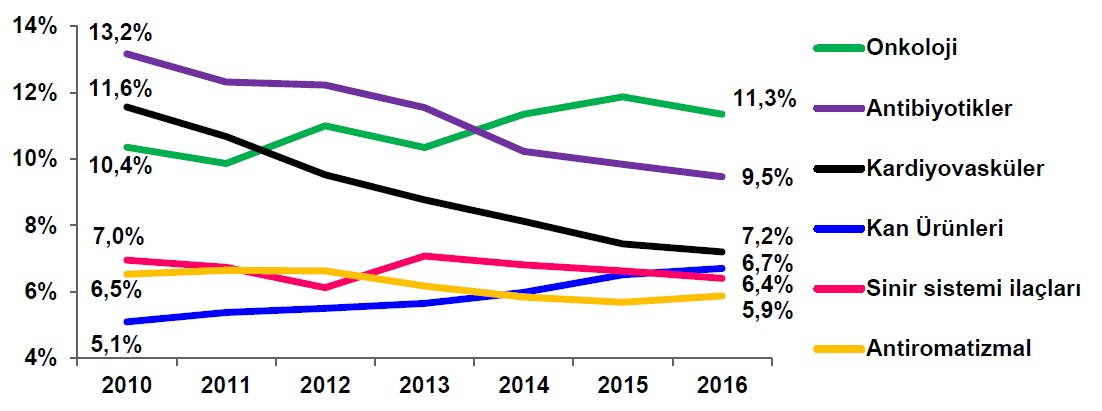
\includegraphics[width=1\linewidth, height=0.15\textheight]{../Figures/eko1}
 	\end{center}
 	  %\vspace{0pt}
 	  \captionof{figure}[İlaçların toplam tutar üzerinden payları]{İlaçların toplam tutar üzerinden payları \cite{sektor17}}
 	  \label{fig:eko1}	
\end{minipage}
\begin{minipage}{0.49\textwidth}
	\begin{center}
	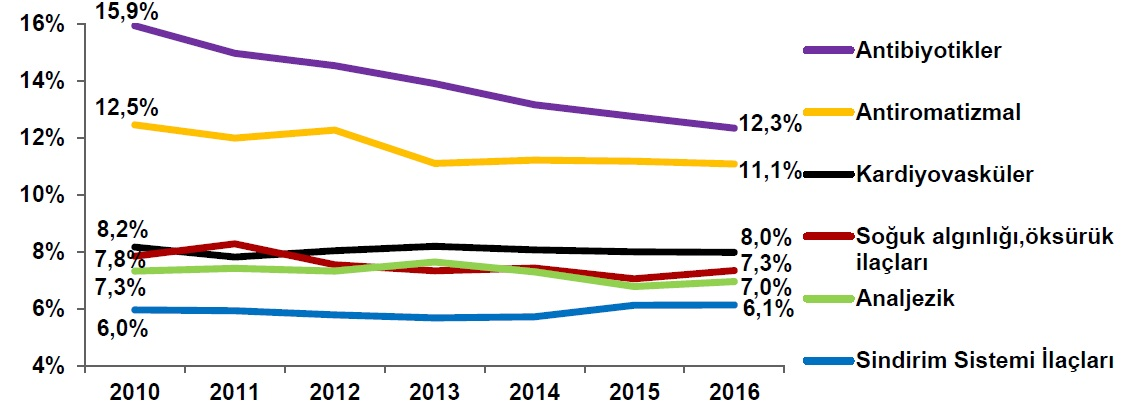
\includegraphics[width=1\linewidth, height=0.15\textheight]{../Figures/eko2}
	\end{center}
	  %\vspace{0pt}
	  \captionof{figure}[İlaçların kutu ölçeğinde payları]{İlaçların kutu ölçeğinde payları \cite{sektor17}}
	  \label{fig:eko2}
\end{minipage}\\



\subsection{Kronik Hepatit B'de Maliyet}

KHB'de en çok hasta yükünü taşıyıcı grup oluşturmaktadır fakat bu grup aynı zamanda KHB hastaları arasında en az harcama yapılan gruptur. Antiviral kullanımı ile ve komplikasyon oluştuğunda kişi başına düşen maliyet artmaktadır. Antiviral ilaç kullanımından fayda görecekleri tanımak komplikasyon gelişme riskini azaltacağından maliyet etkindir. 

Viral hepatit için ilk sırada istenen tarama testlerinin fiyatı 0.5-3 dolardır. Nükleik asit testleri ise 25-200 dolardır \cite{world2017global}. 

Antiviral ilaçlar kullanımıza baktığımızda IMS (Intercontinental Marketing Services) verilerine göre  2017 yılının ilk 6 ayında net kutu bazında satış rakamları şu şekildedir: Tenofovir disoproksil fumarat 290.412; entekavir: 124.912; lamivudin: 59.912; telbivudin: 14.606.  


